\documentclass{article}
\usepackage[a4paper, top=2cm, bottom=2cm, left=2.5cm, right=2.5cm]{geometry}
\usepackage{graphicx}
\usepackage{float}
\usepackage{amsfonts}
\usepackage{amsmath}
\usepackage[dvipsnames]{xcolor}

% Titolo
\title{Appunti di Linguaggi e Tecnologie per il Web}
\author{Federico Falcone}
\date{\today}

\begin{document}

\maketitle
\tableofcontents
\newpage

\section{Networking}
\subsection{Topologie}
Ogni tipologia di rete può essere fisicamente realizata sfruttando topologie differenti:
\begin{itemize}
    \item topologia logica a Bus, cablata a stella
    \begin{figure}[H]
        \centering
        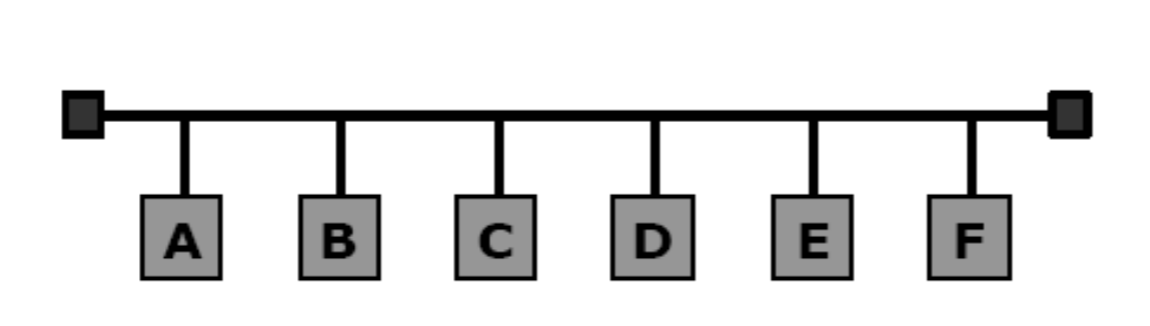
\includegraphics[width=0.4\textwidth]{Images/bus_lineare.png}
    \end{figure}
    \item topologia a stella
    \begin{figure}[H]
        \centering
        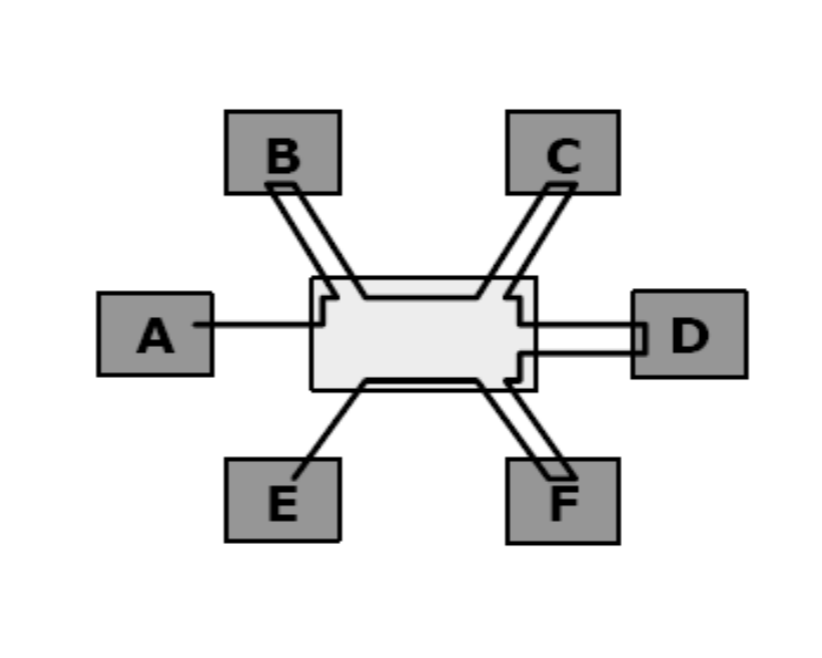
\includegraphics[width=0.4\textwidth]{Images/bus_stella.png}
    \end{figure}
    \item centralizzata
    \begin{figure}[H]
        \centering
        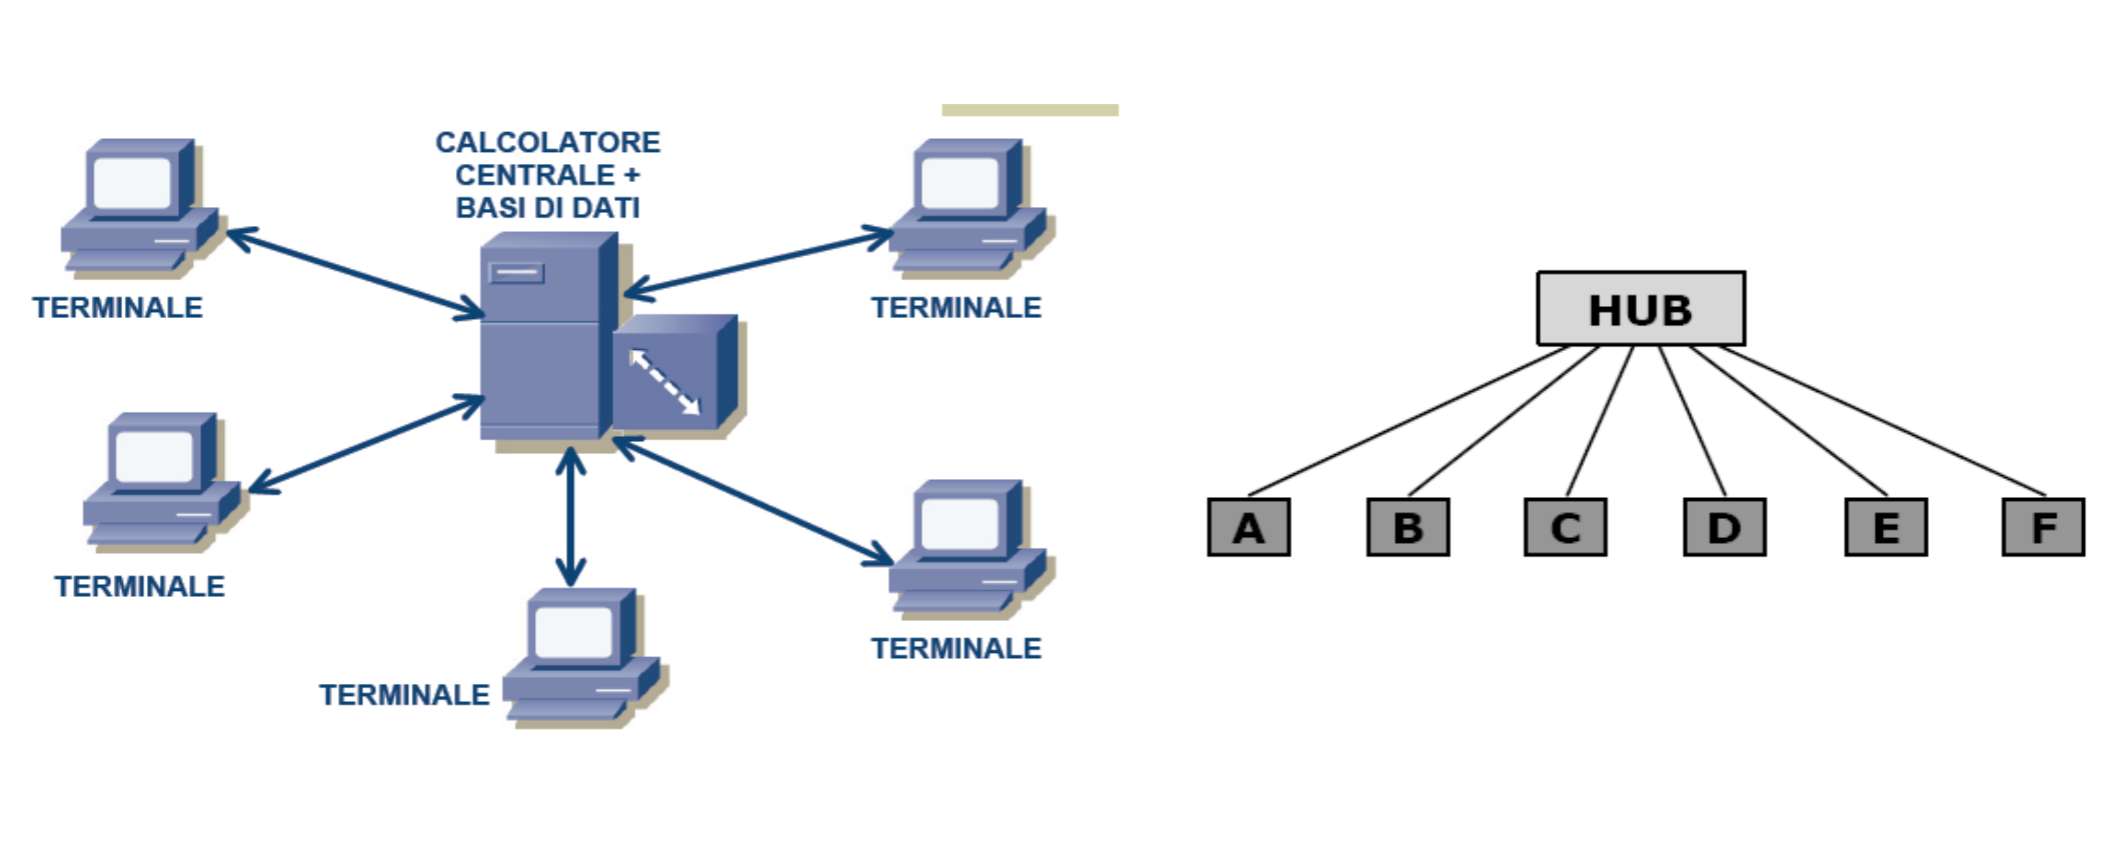
\includegraphics[width=1\textwidth]{Images/centralizzata.png}
    \end{figure}
\end{itemize}

\subsection{Standard}
La comunicazione tra nodi differenti e, possibilmente, basati su piattaforme hardware e/o software eterogenee necessita di \textcolor{red}{standard}.
Storicamente si parla di standard di un produttore: scambio di informazioni possibile solo per sistemi della stessa marca (sistemi \textcolor{red}{chiudi}).
Sono arrivati poi degli standard definiti da enti internazionali (livello di transizione dati).
\\ Il vantaggio è che assicurano un vasto mercato per i dispositivi e il software. Inoltre consentono a prodotti provenienti da fornitori \textcolor{red}{differenti} di comunicare.
\\ Di contro però è una tecnologia congelata e poi posono esserci più standard per la stessa funzione.

\subsubsection{Standard ISO-OSI}
Lo standard ISO ha adottato un modello a strati. Il sistema di comunicazione viene diviso a strati ciascuno dei quali esegue una funzione predefinita.
Strati ISO/OSI possono essere separati in due categorie

\end{document}